% You can define macros here

\title{MWE of SEG abstract}
\author{Thomas Rapstine, Center for Wave Phenomena, Colorado School of Mines}

\maketitle

\section{Introduction}
Introducing the minimum working example.

\section{Theory}
So much theory.
\section{Demonstration}
Here's a short demo of how to use some common features inside of the provided \LaTeX classes.

Equations:
\begin{equation}
    \nabla^2 u - \alpha \frac{\partial u}{\partial t} = 0
\label{eqn:demo}
\end{equation}

Here is how we use equations: ~\ref{eqn:demo}.  Here is how we can make citations \cite[]{godwin_blended_2010,krebs_fast_2009,duquet_3d_1999}. Or we can cite inline as in \cite{godwin_blended_2010}.

We can also make figures using our Madagascar plots.  There are two ways to do so, 1 - using built-in macros and 2 - using the default \LaTeX macros.

The first way:
\inputdir{data}
\plot{noise}{width=0.45\textwidth}{A plot of our signal.}
\sideplot{spectra}{width=0.45\textwidth}{The amplitude spectrum of our signal.}

\multiplot{2}{noise,spectra}{width=0.45\textwidth}{The signal (a), and the amplitude spectrum (b) plotted using multiplot (which is great for making large plots across columns).}

Or we could use includegraphics as usual:

\begin{figure}
    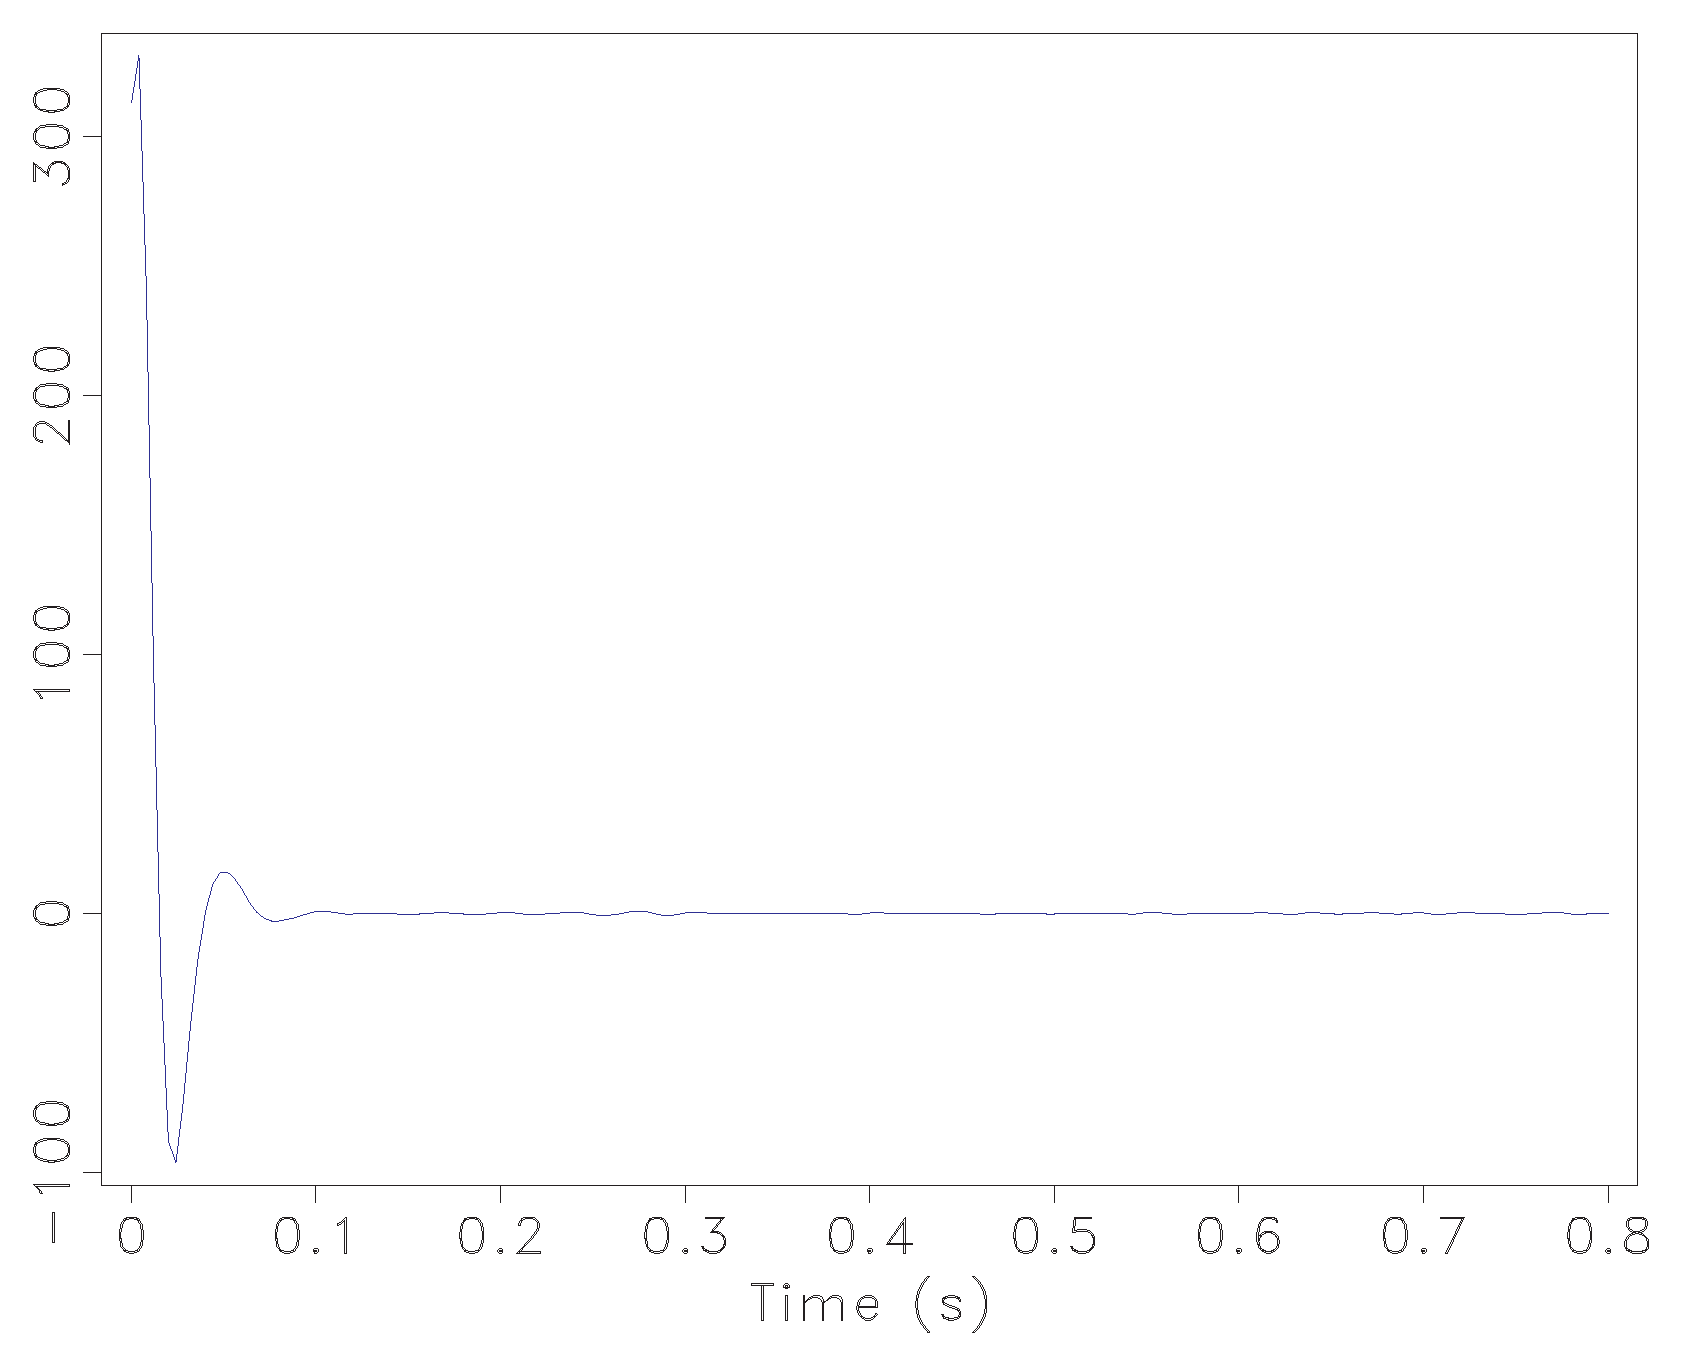
\includegraphics[width=0.45\textwidth]{data/Fig/noise} 
    \caption{The signal.}
\label{Fig:noise}
\end{figure}

\section{Results}
Look, results.

\section{Conclusions}
So many conclusions, so little time.

\bibliographystyle{seg}
\bibliography{demobib}
